\chapter{Serial Verbs}
\label{sec:sv}

In this section I will introduce what I mean when I refer to serial verb constructions (SVCs) in Nuuchahnulth (\S\ref{sec:sv:def}), give the data on the construction (\S\ref{sec:sv:data}), and finally my analysis as implemented in my grammar (\S\ref{sec:sv:analysis}).

\section{Serial Verb Definition} \label{sec:sv:def}

The definition of a serial verb is somewhat contested. In their typological survey, \cite{aikhenvalddixon2006} give several definitions, some of which conflict or overlap. Among their key proposed criteria is multiple verbs that (i) are monoclausal; (ii) from a ``single predicate"; (iii) form a ``single event"; (iv) form one unit phonologically; (v) are negated singly.

Most of these definitions are problematic, however. \citeauthor{aikhenvalddixon2006} give no clear definition for a single predicate or a single event. Without a formal semantic representation, these are left vague, and for the most part a single predicate (when it is not synonymous with a single event) seems to come down to monoclausality. While serial verbs may be phonologically connected, they give several examples where the serial verbs are separated by intervening words (such as a direct object), and give instances of (what they term) serial verbs where one verb is negated while the other is not.

\cite{butt1995} gives an analysis of serialization in Urdu within the structure of Lexical-Functional Grammar (LFG). Since her work is grounded in a specific analysis of a specific language, \citeauthor{butt1995} can be more specific in the definition of a serial verb. A key component of \citeauthor{butt1995}'s analysis is the notion of a ``complex predicate," which is the creation of a new atomic unit of meaning from two separate words. The two components of a complex predicate can have a hierarchical relation in the syntax of the language. The semantic relation for the word `write' might be \textsc{write}(\textit{x}, \textit{y}), but when combined with the permissive, the new semantic relation is \textsc{let-write}(\textit{x}, \textit{y}, \textit{z}), with a syntactic subordination. The predicate composition has created a new, higher-order relation with a different number of arguments, which is necessary in the event that there is evidence (as in Urdu) that the combined verbs have a larger number of arguments than either of the individual verbs.

There are reasons to disprefer this kind of analysis, if possible. One is that this form of complex predicate makes semantic composition much more difficult to model. In the typical lexicalist framework, each content morpheme is associated with an elementary predication, which is a shorthand for the `meaning' of that morpheme, conventionally written as the morpheme in upper-case letters. This convention is for human readability: we could easily label word meanings as \textsc{meaning1647}, \textsc{meaning1648}, etc., with no loss of specificity. \citeauthor{butt1995}'s analysis creates a situation where there is a new mathematical operation in the semantic representation: `let' \textsc{let} + `write' \textsc{write} = \textsc{let-write}. Despite the similarity in labels, there is no formal relationship between these three meaning representations except by that equation, just as if the equation had been \textsc{meaning308} + \textsc{meaning2119} = \textsc{meaning8780}. Even though the meaning is in fact strictly semantically compositional, the meaning representation of the ``complex predicate" is non-compositional in the model with respect to its member verbs.

In some contexts, this is not necessarily a bad thing. Some sort of arbitrariness like this could be used to model idioms, for example [[TODO: find keystone literature on idiom \& multi-word expression from 100 things book]], where individual lexical meanings are non-compositional. However, when this kind of combination is productive (as in the case of serialization), it is preferable not to introduce such semantic non-compositionality, or one ends up with a list of semantic equations, as above, which is nearly the size of the set of verbs in the lexicon (if not larger).

In LFG, the elementary predication of a word is linked to the number of its arguments. That is, the meaning of `write' isn't merely \textsc{write}, but \textsc{write}(\textit{x}, \textit{y}). In this framework, to add an argument to a predication, it is necessary to change the predication itself. In MRS \citep{copestake2005}, the semantic meaning and its arguments are separated from each other. That is, the meaning of `write' is schematized as below:

\begin{avm}
\[ pred & \textsc{write} \\
   arg0 & \textit{e} \\
   arg1 & \textit{x} \\
   arg2 & \textit{y} \\
\]	
\end{avm}

In this way, it is possible to separately alter the number of arguments of the predication \textsc{write} without having to create a new predication. This is something the formalism shares with Neodavidsonian representations \citep{parsons1990}. This difference between the representation \citeauthor{butt1995} uses and and MRS semantic representations will allow me to maintain strict semantic compositionality in my analysis of serial verbs in Nuuchahnulth.

As stated, serial verbs are not clearly defined in the literature, and attempts to generate cross-linguistic definitions quickly run into problems. Even monoclausality, so central to \cite{aikhenvalddixon2006}, is thrown out in \cite{butt1995}, who gives good reasons for syntactic subordination in a structure that otherwise falls into the umbrella of a serialization construction. I will use a very narrow definition of a serial verb construction for Nuuchahnulth. Any clause containing two verbs without an overt coordinator and where the verbs share the semantics of the second position inflectional complex is a clause containing a ``serial verb construction." Each matrix and dependent clause is marked with a second-position clitic, and so the boundaries of a clause are fairly easy to determine.\footnote{The one exception to this is that the third-person neutral mood is null-marked. For this reason, I will use examples that are not in this person-mood combination.} Because of the restriction that serial verb constructions lack an overt coordinator, constructions containing a linker morpheme (\S\ref{sec:link}) do not count as SVCs.

This definition is also restricted to verbs, and not other kinds of multi-predicate constructions. Non-verbs do not participate in the kinds of constructions I will investigate here, and non-verbal multi-predicate constructions are fairly limited in type: they require overt coordination through a coordinand or through a linker construction. The former is outside the scope of this dissertation, and the latter will be addressed in \S\ref{sec:link}.

\subsection{Non-SVCs}

I will give a few examples of common constructions which fall outside my definition of a serial verb construction, although there may be some similarities. The first is juxtaposed clauses (\ref{ex:juxtaposedclauses}).

\ex \label{ex:juxtaposedclauses}
\begingl
\glpreamble hač̓a pawałšiƛ [pause] ʔuušp̓iq [pause] ʔuušp̓iqqač̓a wawaa. //
\gla hač̓a pawał-šiƛ ʔuušp̓iq ʔuušp̓iq=qač̓a wawaa. //
\glb maybe lost-\textsc{mo} something.bad.happens.\textsc{mo} something.bad.happens.\textsc{mo}=\textsc{infr} say.\textsc{cv} //
\glft ` ``Maybe he got lost... something happened... perhaps something happened," they said.' (\textbf{C}, \textit{tupaat} Julia Lucas) //
\endgl
\xe

(\ref{ex:juxtaposedclauses}) comes from a text about a man who was lost at sea and returns. Although one could claim that the first two verbs, \textit{pawałšiƛ} and \textit{ʔuušp̓iq}, are in a SVC, the prosody used in the utterance indicates something else. The repeated \textit{ʔuušp̓iq}, complete with a second position clitic, suggests that these are clauses (the first two under null-marked third person neutral mood) that are adjacent. This kind of structure occurs in speech as people are rephrasing or redescribing an event. (\ref{ex:juxtaposedclauses2}) has the same structure, and is from a description of Raven in a narrative text.

\ex \label{ex:juxtaposedclauses2}
\begingl
\glpreamble ʔayiisšiƛ, hiy̓iisšiƛ haʔumukʔi. //
\gla ʔaya-!iis-šiƛ hiš-!iis-šiƛ haʔum=uk=ʔiˑ //
\glb many-consume-\textsc{mo} all-consume-\textsc{mo} food=\textsc{poss}=\textsc{art} //
\glft `He ate a lot, he ate all of the food.' (\textbf{B}, Marjorie Touchie) //
\endgl
\xe

Like (\ref{ex:juxtaposedclauses}), (\ref{ex:juxtaposedclauses2}) is in the third person, and I believe this is two separate clauses, and not a serialization structure. When these sorts of constructions occur outside the third person, the adjacent clauses require an overt morpheme, and so this apparent ambiguity (serialization vs adjacent clause) does not occur.

The second kind of construction that falls outside my definition of a SVC is Nuuchahnulth temporal expressions. The way to express a duration of time is to juxtapose the time period with the rest of the clause. If the time expression is in the durative aspect, the interpretation is `for \textit{x} time' (\ref{ex:inportforfivedays}). If the time expression is in a perfective aspect, the interpretation is `after \textit{x} time' or `at the end of \textit{x} time' (\ref{ex:afterayear}).

\ex \label{ex:inportforfivedays}
\begingl
\glpreamble suč̓ačłintiis hił c̓uumaʕaas. //
\gla suč̓a-čiˑł=int=(y)iis hił c̓uumaʕaas //
\glb five-day.\textsc{dr}=\textsc{pst}=\textsc{weak.1sg} be.at Port.Alberni //
\glft `I was in Port Alberni for five days.' (\textbf{Q}, Sophie Billy) //
\endgl
\xe

\ex~ \label{ex:afterayear}
\begingl
\glpreamble ʔaḥʔaaʔaƛqač̓a n̓upqʔičḥšiʔeƛ n̓aacsaaƛ ḥiškʷiiʔatḥ č̓apac hintšiƛ ʔuucayu̓k ḥiškʷiiʔatḥ. //
\gla ʔaḥʔaaʔaƛ=qač̓a n̓up-qʔičḥ-šiƛ=!aƛ n̓aacsa=!aƛ ḥiškʷiiʔatḥ č̓apac hintšiƛ ʔu-L.cay̓uk ḥiškʷiiʔatḥ //
\glb and=\textsc{dubv} one-year.\textsc{dr}-\textsc{mo}=\textsc{now} see=\textsc{now} Hesquiaht canoe arrive.\textsc{mo}.\textsc{gr} \textsc{x}-go.\textsc{dr} Hesquiaht //
\glft `And one year later the Hesquiahts saw a boat arriving toward Hesquiaht.' (\textbf{C}, \textit{tupaat} Julia Lucas) //
\endgl
\xe

Although these two types of temporal expression are distinct, it is possible to use the second construction, which uses a perfective form, to express a duration, i.e. \textit{it has become X length of time that Y has been done}, as in \ref{ex:forfourdays}. The opposite (interpreting the durative form to mean `after') is not possible to my knowledge.

\ex \label{ex:forfourdays}
\begingl
\glpreamble ʔaḥʔaaʔaƛ muučiiłšiƛna hił siy̓a ʔaḥʔaaʔaƛ ḥaakʷaaƛuk Matthew, kʷaaʔuucukqs. //
\gla ʔaḥʔaaʔaƛ muu-čiˑł-šiƛ=naˑ hił siy̓a ʔaḥʔaaʔaƛ ḥaakʷaaƛ=uk Matthew kʷaaʔuuc=uk=qs //
\glb and four-day.\textsc{dr}-\textsc{mo}=\textsc{neut.1pl} be.at \textsc{1sg} and young.girl=\textsc{poss} Matthew grandchild=\textsc{poss}=\textsc{defn.1sg} //
\glft `We were there for four days, me and Matthew's daughter, my granddaughter.' (\textbf{C}, \textit{tupaat} Julia Lucas) //
\endgl
\xe

What differentiates these expressions from serial verb constructions, as well as linker constructions (see \S\ref{sec:link}) is the interpretation of the subject. While the temporal component can take the subject-mood portmanteau (\ref{ex:inportforfivedays}, \ref{ex:forfourdays}), the person expressed in the subject clitic is not in any way the subject of the temporal expression. In (\ref{ex:inportforfivedays}), `I' is not the subject of `five days.' This is also the case for the subjects of the verbs in (\ref{ex:afterayear}, \ref{ex:forfourdays}). Instead, the time expression seems to be opaque to the subject information present in the clause. This is not the case for serial verbs, as I will show below.

\section{Data} \label{sec:sv:data}

\subsection{Semantic Types of Serial Verb Constructions}

Descriptively, I categorize observed serial verb constructions into five broad semantic types. These types are not motivated a priori by any external typological theories or a commitment to these categories, but an attempt to make sense of my data. I grouped constructions by words with identical syntactic behavior and tried to create groupings with broad semantic similarities.

\vspace{10pt}

\subsubsection{I. Manner and Action} \label{sec:sv:mannerandaction}

\vspace{10pt}

The broadest semantic type of SVC links actions and manner. By ``manner" what I mean is words that express intention of a main action, or clarify or specify that main action in some way. In Nuuchahnulth, this is typically expressed verbally. I include in this category manner of motion (e.g., go + walk as in \ref{ex:walktoalberni}), emotional affect (e.g., feel-sorry + make-pathetic as in \ref{ex:dontmistreatme}), some kinds of adverbial-like expressions using semantically light verbs like ``do" and ``go ahead" (e.g., only-do + lie-down as in \ref{ex:justliedown}, and go-ahead + go as in \ref{ex:goaheadwent}), and metaphoric motion and action (e.g., go-back + become-alive as in \ref{ex:comebacktolife}).

\ex \label{ex:walktoalberni}
\begingl
\glpreamble \textbf{ʔuucuʔuk}w̓it̓asaḥ \textbf{yaacuk} c̓uumaʕas. //
\gla \textbf{ʔuucuʔuk}-w̓it̓as=(m)aˑḥ \textbf{yaacuk} c̓uumaʕas //
\glb \textbf{go.to.\textsc{dr}}-going.to=\textsc{real.1sg} \textbf{walk.\textsc{dr}} Port.Alberni //
\glft `I'm going to walk to Port Alberni.' (\textbf{B}, Bob Mundy) //
\endgl
\xe

\ex~ \label{ex:dontmistreatme}
\begingl
\glpreamble wik̓iis \textbf{x̣ax̣aał} \textbf{łaakʷiił} siy̓a. //
\gla wik=!iˑs \textbf{x̣ax̣aał} \textbf{łaakʷiił} siy̓a //
\glb \textsc{neg}=\textsc{cmmd.2sg>1sg} \textbf{feel.sorry} \textbf{mistreat} \textsc{1sg} //
\glft `Don't feel sorry for me, mistreating me.' (\textbf{C}, \textit{tupaat} Julia Lucas) //
\endgl
\xe

\ex~ \label{ex:justliedown}
\begingl
\glpreamble \textbf{ʔanasł}intwaʔš \textbf{t̓awiłšƛ}. //
\gla \textbf{ʔana-siła}=int=waˑʔš \textbf{t̓awił-šiƛ} //
\glb \textbf{only-do}=\textsc{pst}=\textsc{hrsy.3} \textbf{lie.down-\textsc{mo}} //
\glft `He just laid down.' (\textbf{Q}, Sophie Billy) //
\endgl
\xe

\ex~ \label{ex:goaheadwent}
\begingl
\glpreamble nay̓iiʔak̓aƛin \textbf{kuw̓iła} \textbf{wałaak}. //
\gla nay̓iiʔak=!aƛ=(m)in \textbf{kuw̓iła} \textbf{wałaak} //
\glb immediately=\textsc{now}=\textsc{real.1pl} \textbf{go.ahead} \textbf{go.\textsc{dr}} //
\glft `We immediately went ahead and went.' (\textbf{B}, Marjorie Touchie) //
\endgl
\xe

\ex~ \label{ex:comebacktolife}
\begingl
\glpreamble \textbf{huʔacači}ʔaqƛsuuk \textbf{tiičačiƛ}. //
\gla \textbf{huʔa-ca-čiƛ}=!aaqƛ=suuk \textbf{tiič-°ačiƛ} //
\glb \textbf{back-go-\textsc{mo}}=\textsc{fut}=\textsc{neut.2pl} \textbf{live-\textsc{in}} //
\glft `You will come back to life.' (\textbf{C}, \textit{tupaat} Julia Lucas) //
\endgl
\xe

This kind of SVC can ``stack" beyond coordinating just two verbs, to at least three.

\ex \label{ex:onlygotostore}
\begingl
\glpreamble \textbf{ʔanasiła}ʔi \textbf{kuw̓iła} \textbf{ʔucačiƛ} makuwił. //
\gla \textbf{ʔana-siła}=!iˑ \textbf{kuw̓iła} \textbf{ʔu-ca-čiƛ} makuwił //
\glb \textbf{only-do}=\textsc{cmmd.2sg} \textbf{go.ahead} \textbf{\textsc{x}-go.to-\textsc{mo}} store //
\glft `Just go to the store.' (\textbf{C}, \textit{tupaat} Julia Lucas) //
\endgl
\xe

\ex \label{ex:movebackucluelet}
\begingl
\glpreamble \textbf{huʔacačiƛ}w̓it̓asaḥ \textbf{šiiƛuk} \textbf{wałaak} yuułuʔiłʔatḥ. //
\gla \textbf{huʔa-ca-čiƛ}-w̓it̓as=(m)aˑḥ \textbf{šiiƛuk} \textbf{wałaak} yuułuʔiłʔatḥ //
\glb \textbf{back-go-\textsc{mo}}-going.to=\textsc{real.1sg} \textbf{move.house.\textsc{dr}} \textbf{go} Ucluelet //
\glft `I'm going to move back to Ucluelet.' (\textbf{B}, Bob Mundy) //
\endgl
\xe

It is possible for one of the verbs and its object (that is, the full VP of one of the serial verbs) to interrupt the other verb and its object, as in (\ref{ex:drivequeenscove}, \ref{ex:takechildrentochurch}).

\ex \label{ex:drivequeenscove}
\begingl
\glpreamble ʔuuct̓iiḥs$_{\text{v\_1}}$ [ƛiḥaa]$_{\text{v\_2}}$ Queens Cove$_{\text{obj\_1}}$. //
\gla ʔuuct̓iiḥ$_{\text{v\_1}}$=s [ƛiḥ-aˑ]$_{\text{v\_2}}$ Queens Cove$_{\text{obj\_1}}$ //
\glb go.toward.\textsc{dr}=\textsc{strg.1sg} drive-\textsc{ct} Queens Cove //
\glft `I am driving to Queens Cove.' (\textbf{N}, Fidelia Haiyupis) //
\endgl
\xe

\ex~ \label{ex:takechildrentochurch}
\begingl
\glpreamble hiniicintiisʔinł$_{\text{v\_1}}$ [ʔucičƛ$_{\text{v\_2}}$ ciquuwłi$_{\text{obj\_2}}$]$_{\text{vp\_2}}$ t̓aatn̓aʔiskqs$_{\text{obj\_1}}$. //
\gla hina-iic$_{\text{v\_1}}$=int=(y)iis=ʔinł [ʔu-ci-čiƛ$_{\text{v\_2}}$ ciq-uwił=ʔiˑ$_{\text{obj\_2}}$]$_{\text{vp\_2}}$ L.<t>-t̓an̓a=ʔis=uk=qaˑs$_{\text{obj\_1}}$  //
\glb \textsc{empty}-carry=\textsc{pst}=\textsc{weak.1sg}=\textsc{habit} \textsc{x}-go.to-\textsc{mo} pray-building \textsc{pl}-child=\textsc{dimin}=\textsc{poss}=\textsc{defn.1sg} //
\glft `I would always take my children to church.' (\textbf{Q}, Sophie Billy) //
\endgl
\xe

The verbs in this type of SVC, for most speakers, must agree in perfectiveness. Nuuchahnulth has a great many verbal aspect markers which follow the root, but they can be broken into two categories: perfective aspect (momentaneous and inceptive) and imperfective aspect (continuative, durative, repetitive, iterative, and graduative). The derivations in (\ref{aspect}) give a simplified view of my understanding of how these aspects are related to each other. Much of this is taken from \cite{davidson2002}, as well as personal correspondence with Davidson, who deserves much credit for working out this system. My understanding of the inceptive as underlyingly continuative + perfective is indebted to Werle.\footnote{Note that this means that the morphology for the continuative and inceptive do not ``stack," unlike the other aspect forms. So momentaneous + graduative is realized as \textit{-šiƛ} and also a long-short template. However continuative + inceptive is simply \textit{-°iˑčiƛ}, not *\textit{-aˑ-°iˑčiƛ}. In my implementation, I treat the inceptive as a fully separate aspect, although I believe it is conceptually continuous + perfective.} To simplify the graph, I have combined repetitive-perfective, graduative-perfective, and iterative-perfective into a single node, since verbs in this form cannot undergo further aspectual change.

\begin{comment}
\ex \label{aspect}
\vspace{-20pt}
\xe
\begin{tikzpicture}[sibling distance=10em,
  every node/.style = {shape=rectangle, align=center}]]
\node (root) at (8,4.5) {Root};
\node (mo) at (2,2) {Momentaneous};
\node (ct) at (6,2) {Continuative};
\node (dr) at (8.5,2) {Durative};
\node (rp) at (12,2) {Repetitive};
\node (it) at (15,2) {Iterative};
\node (in) at (2, 0) {Inceptive};
\node (gr) at (5.5, 0) {Graduative};
\node (pf) at (2, -2) {*-Perfective};
\node (*pf) at (15, -2.14) {};
\draw[->] (root) -- (mo) node[midway,fill=white] {-šiƛ};
\draw[->] (root) -- (ct) node[midway,fill=white] {-aˑ};
\draw[->] (root) -- (dr) node[midway,fill=white] {-uk/-L.ḥi};
\draw[->] (root) -- (rp) node[midway,fill=white] {-LR2L.a};
\draw[->] (root) -- (it) node[midway,fill=white] {-LR2L.š};
\draw[->] (mo) -- (gr) node[near start,fill=lightgray] {-LS};
\draw[->] (in) -- (gr) node[near start,fill=lightgray] {-LS};
\draw[->] (ct) -- (in) node[near start,fill=white] {-°iˑčiƛ};
\draw[->] (dr) -- (gr) node[midway,fill=white] {-LS};
\draw[->] (gr) -- (pf) node[near end,fill=lightgray] {-šiƛ};
\begin{scope}[on background layer]
\node[bigbox, fit=(ct)(dr)(it)(gr)(*pf), fill=white] (impf) {};
\node[below left] at (impf.north east) {\textit{imperfective aspect}};
\node[bigbox, fit=(mo)(pf), fill=lightgray] (perf) {};
\node[below right] at (perf.north west) {\textit{perfective aspect}};
\draw[->] (rp) -- (pf);
\draw[->] (it) -- (pf);
%\draw[->] (it) to [out=150,in=30] (pf);
\draw[->] (dr) -- (pf);
\end{scope}
\end{tikzpicture}
\end{comment}

\ex \label{aspect}
\vspace{-20pt}
\xe
\begin{tikzpicture}[sibling distance=10em,
  every node/.style = {shape=rectangle, align=center}]
\node (root) at (8,4.5) {Root};
\node (mo) at (2,2) {Momentaneous};
\node (ct) at (8,2) {Continuative};
\node (dr) at (10.5,2) {Durative};
\node (rp) at (13,2) {Repetitive};
\node (it) at (15,2) {Iterative};
\node (in) at (4.5,2) {Inceptive};
\node (mo-grad) at (2,0) {moment.-grad.};
\node (in-grad) at (4.5,0) {incept.-grad.};
\node (dr-grad) at (10.5,0) {durative-grad.};
\node (mo-grad-pf) at (2,-2) {mom.-grad.-perf.};
\node (in-grad-pf) at (4.5,-2) {inc.-grad.-perf.};
\node (dr-pf) at (7,-2) {durative-grad.};
\node (dr-grad-pf) at (10.5,-2) {dur.-grad.-perf.};
\node (rp-pf) at (13,-2) {repet.-perf.};
\node (it-pf) at (15,-2) {iter.-perf.};
\draw[->] (root) -- (mo) node[midway,fill=white] {-šiƛ};
\draw[->] (root) -- (ct) node[midway,fill=white] {-aˑ};
\draw[dashed,->] (root) -- (in) node[midway, fill=white] {-°iˑčiƛ};
\draw[->] (ct) -- (in);
\draw[->] (root) -- (dr) node[midway,fill=white] {-uk};
\draw[->] (root) -- (rp) node[midway,fill=white] {-LR2L.a};
\draw[->] (root) -- (it) node[midway,fill=white, right] {-LR2L.š};
\draw[->] (mo) -- (mo-grad) node[near start,fill=lightgray] {-LS};
\draw[->] (in) -- (in-grad) node[near start,fill=lightgray] {-LS};
\draw[->] (dr) -- (dr-grad) node[midway,fill=white] {-LS};
\draw[->] (mo-grad) -- (mo-grad-pf) node[near start,fill=white] {-šiƛ};
\draw[->] (in-grad) -- (in-grad-pf) node[near start,fill=white] {-šiƛ};
\draw[->] (dr) -- (dr-pf) node[midway,fill=white] {-šiƛ};
\draw[->] (dr-grad) -- (dr-grad-pf) node[near start,fill=white] {-šiƛ};
\draw[->] (rp) -- (rp-pf) node[midway,fill=white] {-šiƛ};
\draw[->] (it) -- (it-pf) node[midway,fill=white] {-šiƛ};
\begin{scope}[on background layer]
\node[draw=none, fit=(ct)(dr)(it)(dr-grad), fill=white] (impf) {};
\node[above left] at (impf.north east) {\textit{imperfective}};
\node[bigbox, fit=(mo)(in), fill=lightgray] (perf) {};
\node[below right] at (perf.north west) {\textit{perfective}};
\node[bigbox, fit=(mo-grad-pf)(it-pf), fill=lightgray] (perf2) {};
\node[below right] at (perf2.north west) {\textit{perfective}};
%\draw[->] (rp) -- (pf);
%\draw[->] (it) -- (pf);
%\draw[->] (it) to [out=150,in=30] (pf);
%\draw[->] (dr) -- (pf);
\end{scope}
\end{tikzpicture}

\begin{comment}
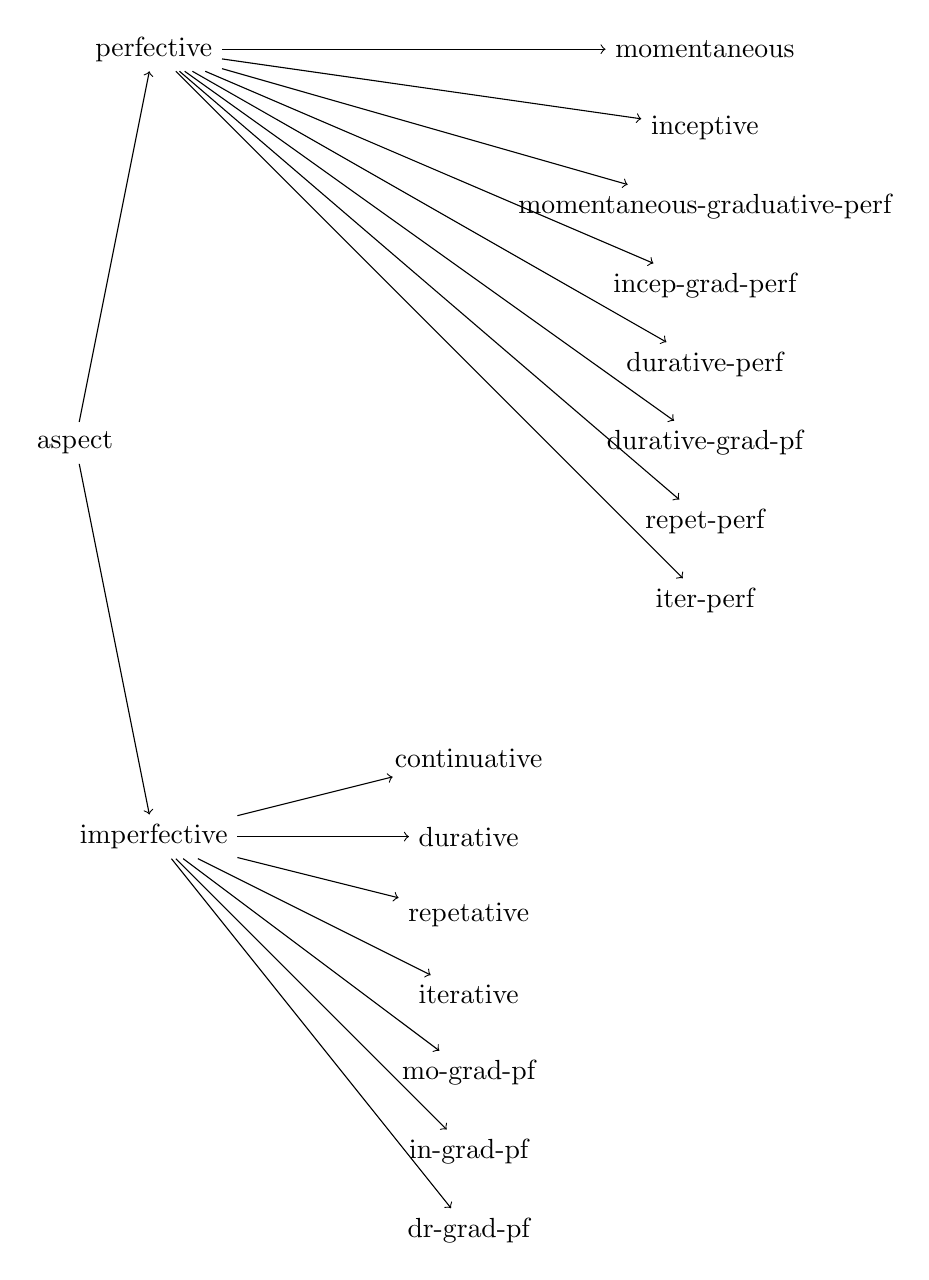
\begin{tikzpicture}[sibling distance=10em,
  every node/.style = {shape=rectangle, align=center}]
\node (aspect) at (0,10) {aspect};
\node (pf) at (1,15) {perfective};
\node (impf) at (1,5) {imperfective};
\node (mo) at (8,15) {momentaneous};
\node (in) at (8,14) {inceptive};
\node (mo-grad-pf) at (8,13) {momentaneous-graduative-perf};
\node (in-grad-pf) at (8,12) {incep-grad-perf};
\node (dr-pf) at (8,11) {durative-perf};
\node (dr-grad-pf) at (8,10) {durative-grad-pf};
\node (rp-pf) at (8,9) {repet-perf};
\node (it-pf) at (8,8) {iter-perf};
\node (ct) at (5,6) {continuative};
\node (dr) at (5,5) {durative};
\node (rp) at (5,4) {repetative};
\node (it) at (5,3) {iterative};
\node (mo-grad) at (5,2) {mo-grad-pf};
\node (in-grad) at (5,1) {in-grad-pf};
\node (dr-grad) at (5,0) {dr-grad-pf};
\draw[->] (aspect) -- (pf);
\draw[->] (aspect) -- (impf);
\draw[->] (pf) -- (mo);
\draw[->] (pf) -- (in);
\draw[->] (pf) -- (mo-grad-pf);
\draw[->] (pf) -- (in-grad-pf);
\draw[->] (pf) -- (dr-pf);
\draw[->] (pf) -- (dr-grad-pf);
\draw[->] (pf) -- (rp-pf);
\draw[->] (pf) -- (it-pf);
\draw[->] (impf) -- (ct);
\draw[->] (impf) -- (dr);
\draw[->] (impf) -- (rp);
\draw[->] (impf) -- (it);
\draw[->] (impf) -- (mo-grad);
\draw[->] (impf) -- (in-grad);
\draw[->] (impf) -- (dr-grad);
\end{tikzpicture}
\end{comment}

\vspace{10pt}

The requirements on SVC aspectual agreement only seem to extend to the level of perfective vs imperfective. In (\ref{ex:goingtoucluelet}), the two verbsare both in the durative aspect. In the ungrammatical \ref{ex:*goingtoucluelet}, the second verb has been moved to the momentaneous, which is a perfective aspect, and mismatches with the first verb, which remains in an imperfective aspect.

\ex \label{ex:goingtoucluelet}
\begingl
\glpreamble ʔuuciy̓ukw̓it̓ass yuułuʔiłʔatḥ yaacuk. //
\gla ʔuuciy̓uk-w̓it̓as=s yuułuʔiłʔatḥ yaacuk //
\glb go.\textsc{dr}-going.to=\textsc{strg.1sg} Ucluelet walk.\textsc{dr} //
\glft `I'm going to walk to Ucluelet.' (\textbf{C}, \textit{tupaat} Julia Lucas) //
\endgl
\xe

\ex~ \label{ex:*goingtoucluelet}
\begingl
\glpreamble *ʔuuciy̓ukw̓it̓ass yuułuʔiłʔatḥ yaacšiƛ. //
\gla ʔuuciy̓uk-w̓it̓as=s yuułuʔiłʔatḥ yaacšiƛ //
\glb go.\textsc{dr}-going.to=\textsc{strg.1sg} Ucluelet walk.\textsc{pf} //
\glft Intended: `I'm going to walk to Ucluelet.' (\textbf{C}, \textit{tupaat} Julia Lucas) //
\endgl
\xe

(\ref{ex:drivehome}) and (\ref{ex:*drivehome}) show the same pattern. In (\ref{ex:drivehome}), the first verb \textit{ƛiḥaa} is in the continuative aspect, which is imperfective, and the second verb \textit{waałšiƛ} is in graduative, which is also imperfective. In (\ref{ex:*drivehome}), the same two verb roots are used, but instead of imperfective, graduative \textit{waałšiƛ}, there is momentaneous, perfective \textit{wałšiƛ}. This aspectual mismatch causes (\ref{ex:*drivehome}) to be ungrammatical.

[[TODO: CHANGE BASED ON 3/24 SESSION]]

\ex \label{ex:drivehome}
\begingl
\glpreamble ƛiḥaamitniš siy̓a łuučm̓uupukqs waałšiƛ. //
\gla ƛiḥ-aˑ=(m)it=niˑš siy̓a łuučm̓uup=uk=qs wał-šiƛ-LS //
\glb drive-\textsc{ct}=\textsc{pst}=\textsc{strg.1pl} \textsc{1sg} sister=\textsc{poss}=\textsc{defn.1sg} go.home-\textsc{mo}-\textsc{gr} //
\glft `We were driving home in the car.' (\textbf{C}, \textit{tupaat} Julia Lucas) //
\endgl
\xe

\ex~ \label{ex:*drivehome}
\begingl
\glpreamble *wałšiƛw̓it̓asniš ƛiḥaa. //
\gla wał-šiƛ-w̓it̓as=niˑš ƛiḥ-aˑ //
\glb go.home-\textsc{mo}-going.to=\textsc{strg.1pl} drive-\textsc{ct} //
\glft Intended: `We will drive home.' (\textbf{C}, \textit{tupaat} Julia Lucas) //
\endgl
\xe

However, for one of my consultants, Sophie Billy, who is the youngest speaker, the only Checkleseht speaker I worked with, and typically the most innovative in her speech patterns, the verbs in this kind of SVC may differ in aspect. I do not know if this is a Checkleseht feature, a Kyuquot-Checkleseht feature, a feature of her generation, or a feature of her idiolect. But this pattern is productive for her.

\ex \label{ex:movetovictoria1}
\begingl
\glpreamble ʔucičƛiis šiiƛuk mituunii. //
\gla ʔu-ci-čiƛ=(y)iis šiiƛuk mituunii  //
\glb \textsc{x}-go-\textsc{mo}=\textsc{weak.1sg} move.house.\textsc{dr} Victoria //
\glft `I moved to Victoria.' (\textbf{Q}, Sophie Billy) //
\endgl
\xe

[[TODO: šiiƛuk is ambiguous between PF and IMPF, so don’t use it, use one of SB’s other examples.]]

\ex~ \label{ex:movetovictoria2}
\begingl
\glpreamble ʔuuct̓iiḥiis šiiƛuk mituunii. //
\gla ʔuuct̓iiḥ=(y)iis šiiƛuk mituunii  //
\glb go.\textsc{dr}=\textsc{weak.1sg} move.house.\textsc{dr} Victoria //
\glft `I moved to Victoria.' (\textbf{Q}, Sophie Billy) //
\endgl
\xe

\begin{comment}
Ordering preference. One of my speakers expressed a strong preference for the manner verb to precede the action. This mirrors how adverbs are used in Nuuchahnulth, which also tend to precede the verb. Other speakers I consulted with were comfortable with the verbs coming in either order.

\ex \label{ex:gohomedrive}
\begingl
\glpreamble ʔucičƛsiš šiiƛuk mituuni. //
\gla ʔu-ci-čiƛ=siˑš šiiƛuk mituuni  //
\glb \textsc{x}-go-\textsc{mo}=\textsc{strg.1sg} move.house-\textsc{dr} Victoria //
\glft `I moved to Victoria.' (\textbf{Q}, Sophie Billy) //
\endgl
\xe
FH
*waałšiʔaƛs ƛiiƛiiḥataḥ.
waałšiʔaƛs. ƛiiƛiiḥataḥʔaƛs.
\end{comment}

\vspace{10pt}

\subsubsection{II. Location and Action}

\vspace{10pt}

Perhaps the most common semantic type of serialization is location-action. Most descriptive locations in Nuuchahnulth are verbs, `be at a place' and locations are simply juxtaposed with the action performed there. This strategy is used for transitive \textit{hił} `be at' as well as intransitive locations like \textit{hitaas} or \textit{ƛ̓aaʔaas} `be outside' and \textit{hitinqis} `be at the beach.'

\ex \label{ex:stopthere}
\begingl
\glpreamble hiłʔii wiinapuƛ. //
\gla hił=!iˑ wiinapuƛ //
\glb be.at=\textsc{cmmd.2sg} stop.\textsc{mo} //
\glft `Stop there.' (\textbf{B}, Bob Mundy) //
\endgl
\xe

\begin{comment}
\ex \label{ex:workathome}
\begingl
\glpreamble hiłitin maḥt̓iiʔakqas mamuuk. //
\gla hił=(m)it=(m)in maḥt̓ii=ʔak=qaˑs mamuuk //
\glb be.at=\textsc{pst}=\textsc{strg.1pl} house=\textsc{poss}=\textsc{defn.1sg} work.\textsc{dr} //
\glft `We worked at my house.' (\textbf{N}, Fidelia Haiyupis) //
\endgl
\xe

\ex \label{ex:screamatbeach}
\begingl
\glpreamble n̓aʔiičiʔeƛ naʔuu łuucma ʕiikʕiika hitinqis. //
\gla n̓a-°iˑčiƛ=!aƛ naʔuu łuucma ʕik-LR2L.a hitinqis //
\glb see-\textsc{in}=\textsc{now} be.with woman=\textsc{poss} scream-\textsc{rp} be.at.beach //
\glft `He heard a woman screaming on the beach.' (\textbf{C}, \textit{tupaat} Julia Lucas) //
\endgl
\xe
\end{comment}


\ex~ \label{ex:speakoutside}
\begingl
\glpreamble hitaasitaḥ ciiqciiqa. //
\gla hitaas=(m)it=(m)aˑḥ ciq-LR2L.a //
\glb be.outside=\textsc{pst}=\textsc{real.1sg} speak-\textsc{rp} //
\glft `I was outside speaking.' (\textbf{B}, Bob Mundy) //
\endgl
\xe

\begin{comment}
\ex~ \label{ex:speakoutside}
\begingl
\glpreamble qiiʔaƛintiis mamuuk ƛ̓aaʔaas. //
\gla qii=!aƛ=int=iis mamuuk ƛ̓aaʔaas //
\glb long.time=\textsc{now}=\textsc{pst}=\textsc{weak.1sg} work.\textsc{dr} be.outside //
\glft `I was working outside for a long time.' (\textbf{Q}, Sophie Billy) //
\endgl
\xe

\ex~ \label{ex:hideonroof}
\begingl
\glpreamble haptsaapaqƛiis suutił hiłaayiłkʷ. //
\gla hapt-saˑp=ʔaqƛ=iis sut-L.(č)ił hił-aˑyił=uk. //
\glb hide-\textsc{mo.caus}=\textsc{fut}=\textsc{weak.1sg} \textsc{2sg}-do.to be.at-on.a.roof=\textsc{poss} //
\glft `I will hide you on the roof.' (\textbf{Q}, Sophie Billy) //
\endgl
\xe
\end{comment}

As with Type I, it is possible in this construction for the transitive location verb \textit{hił} `be at' to be split from its object by the other verb (\ref{ex:restonmountains}), or the other verb and its object (\ref{ex:sawbearonmountain}).

\ex \label{ex:restonmountains}
\begingl
\glpreamble hiłqiimitʔišʔał huuxsʔatu nučii. //
\gla hił-qii=(m)it=ʔiˑš=ʔaˑł huuxsʔatu nuč-iˑ //
\glb be.at-on.top=\textsc{pst}=\textsc{strg.3}=\textsc{habit} rest.\textsc{dr} mountain-\textsc{nmlz} //
\glft `He rests on top of mountains.' (\textbf{N}, Fidelia Haiyupis) //
\endgl
\xe

\ex \label{ex:sawbearonmountain}
\begingl
\glpreamble hiłqiiʔaƛin n̓aacsiičiƛ čums nučii. //
\gla hił-qii=!aƛ=in n̓aacs-°iˑčiƛ čums nuč-iˑ //
\glb be.at-on.top=\textsc{now}=\textsc{weak.1pl} see-\textsc{in} bear mountain-\textsc{nmlz} //
\glft `We saw a bear (we being) on top of the mountain.' (\textbf{N}, Fidelia Haiyupis) //
\endgl
\xe

\begin{comment}
\ex~ \label{ex:hiddeninthewall}
\begingl
\glpreamble huptsaapckʷaƛ hinałc̓ił ʔiiḥmisukʔi p̓atquk. //
\gla hupt-saˑp=ckʷiˑ=!aƛ hina-ałc̓ił ʔiiḥmis=uk=ʔiˑ p̓atquk //
\glb hide-\textsc{mo.caus}=remains.of=\textsc{now} \textsc{empty}-in.wall important=\textsc{poss}=\textsc{art} belongings //
\glft `They hid their belongings in the walls.' (\textbf{B}, Bob Mundy) //
\endgl
\xe
\end{comment}

\begin{comment}
This ``interruption" can occur the other way around, when the location word is intransitive.

\ex \label{ex:gasolinebydoor}
\begingl
\glpreamble ḥuqšiƛ ʔucačiƛ ḥaa yaqʔiitq hiiłsʔat̓uus gasoline.\footnotemark //
\gla ḥuq-šiƛ ʔu-ca-čiƛ ḥaa yaq=ʔiˑtq hił-L.sʔat̓uus gasoline //
\glb tip.over-\textsc{mo} \textsc{x}-go-\textsc{mo} who.what=\textsc{defn.3} be.at-by.the.door gasoline //
\glft `It knocked the gasoline over toward the door..' (\textbf{C}, \textit{tupaat} Julia Lucas) //
\endgl
\xe

\footnotetext{In this dependent construction, `gasoline' is the participant of the predicative relativizer \textit{yaq} `who'. The bracketing is [ḥuqšiƛ ʔucačiƛ]\textsubscript{pred} [ḥaa [yaqʔiitq hiiłsʔat̓uus gasoline] ]\textsubscript{part}}
\end{comment}

Unlike Type I SVCs, there is no requirement that the verbs match in their aspect. This is partly because most locatives do not inflect for aspect. For the basic verb \textit{hił} `be at' there is no perfective form of \textit{hiłšiƛ}, and \textit{hił} can serialize with both perfective (\ref{ex:stopthere}) and imperfective verbs (\ref{ex:restonmountains}). There exist perfective forms for some of the other location words, for instance \textit{hitinqsaƛ} `go to the beach' from \textit{hitinqis} `be at the beach.' However, there is no requirement for aspectual agreement here, as these location verbs can serialize with both perfective (\ref{ex:sawbearonmountain}) and imperfective verbs (\ref{ex:speakoutside}).

Unlike Type I verbs, there is a strict ordering requirement. The location verb must always come before the action verb (\ref{ex:outsidespeaking}, \ref{ex:*outsidespeaking}). 

\ex \label{ex:outsidespeaking}
\begingl
\glpreamble hitaasitaḥ ciiqciiqa. //
\gla hitaas=(m)it=(m)aˑḥ ciq-LR2L.a  //
\glb outside-\textsc{pst}=\textsc{real.1sg} speak-\textsc{rp} //
\glft `I was speaking outside.' (\textbf{B}, Bob Mundy) //
\endgl
\xe

[[TODO: You forgot to change this to =imt, that may be why bob rejected it, find other ex. or retry with Bob ]]

\ex~ \label{ex:*outsidespeaking}
\begingl
\glpreamble *ciiqciiqamitaḥ hitaas. //
\gla ciq-LR2L.a=(m)it=(m)aḥ hitaas  //
\glb speak-\textsc{rp}=\textsc{pst}=\textsc{real.1sg} outside //
\glft Intended: `I was speaking outside.' (\textbf{B}, Bob Mundy) //
\endgl
\xe

\ex~ \label{ex:workathome}
\begingl
\glpreamble hiłʔaƛin mamuuk wałyookqs. //
\gla hił=!aƛ=in mamuuk wałyuu=ʔak=qaˑs  //
\glb be.at=\textsc{now}=\textsc{strg.1sg} work.\textsc{dr} home=\textsc{poss}=\textsc{defn.1sg} //
\glft `We are working at my home.' (\textbf{Q}, Sophie Billy) //
\endgl
\xe

\ex~ \label{ex:*workathome}
\begingl
\glpreamble *mamuuk̓ƛin hił wałyookqs. //
\gla mamuuk=!aƛ=in hił wałyuu=ʔak=qaˑs  //
\glb work=\textsc{now}=\textsc{strg.1sg} be.at home=\textsc{poss}=\textsc{defn.1sg} //
\glft Intended: `We are working at my home.' (\textbf{Q}, Sophie Billy) //
\endgl
\xe

[[TODO: Are these the best ex's? Comes from a long session with FH, might have been fatigued about linker questions]]

\ex~ \label{ex:shoutoutside}
\begingl
\glpreamble ƛ̓aaʔaasči ʕaaqʕaaqa. //
\gla ƛ̓aaʔaas=či ʕaq-LR2L.a  //
\glb outside=\textsc{cmgo.2sg} yell-\textsc{ro} //
\glft `Go yell outside.' (\textbf{N}, Fidelia Haiyupis) //
\endgl
\xe

\ex~ \label{ex:*singoutside}
\begingl
\glpreamble *nunuukči ƛaaʔaas. //
\gla nunuuk=či ƛaaʔaas  //
\glb sing.\textsc{dr}=\textsc{cmgo.2sg} outside //
\glft Intended: `Go sing outside.'\footnotemark{} (\textbf{N}, Fidelia Haiyupis) //
\endgl
\xe

\footnotetext{(\ref{ex:*singoutside}) can be ``saved" by adding a linker to the location, i.e. \textit{nunuukči ƛ̓aaʔaasḥ}. This creates a new type of construction, which I will discuss in \S\ref{sec:link}.}

%However, he did spontaneously generate the ``ungrammatical" ordering of action-location in running text in ex (\ref{ex:hiddeninthewall}). My interpretation of this is that there is a strong preference for the locative verb to come first, although it may not be strictly ungrammatical. Elder Fidelia Haiyupis (Northern dialect) agreed with Bob's judgments, while other consultants accepted either ordering.
%NB: This is actually a headless relative, which apparently only hił can do, or it may (less likely?) be a complement of hide. This does not occur in any other contexts.

One of my speakers, \textit{tupaat} Julia Lucas did accept, under elicitation and after dealing with many such constructions over many sessions, sentences like (\ref{ex:*outsidespeaking}, \ref{ex:*workathome}, \ref{ex:*singoutside}). However, she has never produced utterances of this type in any texts I have collected from her, and my earlier elicitation work had her rejecting these sentences. Julia is a language instructor, and my interpretation is that she was being accommodating toward my bad Nuuchahnulth at the margins of grammar in her role as a language revitalizer.

This restriction on location-action serialization can be interpreted as a grammaticalization of a larger preference in Nuuchahnulth for modifying expressions to precede what they modify. For instance, adverbs will preferentially precede the verb (and speakers will correct themselves and others by moving adverbs before to a verb). But unlike this type of serialization adverbs can in the right circumstances occur post-verbally.

\vspace{10pt}

\subsubsection{III. Adpositive-like verbs}

\vspace{10pt}

A fuller discussion of adpositive-like words will have to wait for \S\ref{sec:link:adpositive}. It is enough here to mention that, according to the analysis in \citep{woo2007b}, a series of words with meanings that in English are expressed with prepositions are, in Nuuchahnulth, expressed with verbs (\ref{ex:usechair}, \ref{ex:withsistergo}). This includes verbs with basic commative, benefactive, and instrumentive meanings. These constructions have the same property of the above SVCs, where an intransitive verb may ``interrupt" a transitive verb (in this case, the adpositive-like verb) and its object (\ref{ex:workfortrudeau}).


\ex \label{ex:usechair}
\begingl
\glpreamble hiinasinƛayaʔiš haw̓acsac̓umʔi ʔuuḥw̓ał kʷaacsac̓um. //
\gla hiinasinƛ-aya=ʔiˑš haw̓acsac̓um=ʔiˑ ʔu-L.ḥw̓ał kʷaacsac̓um //
\glb climb-\textsc{ct}=\textsc{strg.3sg} table=\textsc{art} \textsc{x}-use chair //
\glft `Using the chair he climbed onto the table.' (\textbf{N}, Fidelia Haiyupis) //
\endgl
\xe

\ex~ \label{ex:withsistergo}
\begingl
\glpreamble ʔuupaałw̓it̓asniš y̓ukʷiiqsu ʔucačiƛ Campbell River. //
\gla ʔuupaał-w̓it̓as=niˑš y̓ukʷ-iˑqsu ʔu-ca-čiƛ Campbell River //
\glb with-going.to=\textsc{strg.1pl} younger.sibling-relation \textsc{x}-go.to-\textsc{mo} Campbell River //
\glft `I'm going with my younger sister to Campbell River.' (\textbf{C}, \textit{tupaat} Julia Lucas) //
\endgl
\xe

\ex~ \label{ex:workfortrudeau}
\begingl
\glpreamble ʔucḥins mamuuk Trudeau. //
\gla ʔu-cḥin=s mamuuk Trudeau //
\glb \textsc{x}-do.for=\textsc{strg.1sg} work.\textsc{dr} Trudeau //
\glft `I'm working for Trudeau.' (\textbf{N}, Fidelia Haiyupis) //
\endgl
\xe

None of the adpositive-like verbs inflect for aspect, and in this way are similar to the locative verb \textit{hił}. Like \textit{hił} and like Type II SVCs, adpositive-likes can serialize with both perfective (\ref{ex:withsistergo}, \ref{ex:goingwithfriend}) and imperfective verbs (\ref{ex:usechair}, \ref{ex:workfortrudeau}). Unlike Type I and II SVCs, the ``interrupting verb phrase" cannot be a transitive verb with its argument.

\ex \label{ex:goingwithfriend}
\begingl
\glpreamble ʔucačiʔaƛukʷitaḥ t̓an̓eʔis c̓uumaʕas ʔukʷink yaqsčaʕinʔitq. //
\gla ʔu-ca-čiƛ=!aƛ=uk=(m)it=(m)aḥ t̓an̓a=ʔis c̓uumaʕas ʔu-(č)ink yaq-sčaʕin=ʔiˑtq //
\glb \textsc{x}-go-\textsc{mo}=\textsc{now}=\textsc{poss}=\textsc{pst}=\textsc{real.1sg} child=\textsc{dimin} Port.Alberni \textsc{x}-with who-friendly=\textsc{defn.3} //
\glft `My child went to Port Alberni with his friend.' (\textbf{B}, Bob Mundy) //
\endgl
\xe

\ex~ \label{ex:*goingwithfriend}
\begingl
\glpreamble *ʔukʷink̓aƛukʷitaḥ ʔucačiƛ t̓an̓eʔis yaqsčaʕinʔitq. //
\gla ʔu-(č)ink=!aƛ=uk=(m)it=(m)aḥ ʔu-ca-čiƛ t̓an̓a=ʔis yaq-sčaʕin=ʔiˑtq //
\glb \textsc{x}-with=\textsc{now}=\textsc{poss}=\textsc{pst}=\textsc{real.1sg} \textsc{x}-go-\textsc{mo} child=\textsc{dimin} who-friendly=\textsc{defn.3} //
\glft Intended: `My child went with his friend.' (\textbf{B}, Bob Mundy) //
\endgl
\xe

%ʔukʷinkw̓it̓asaḥ mituuni wałaak yaqsčaʕinakqas

\vspace{10pt}

\subsubsection{IV. Transitive-Intransitive Repetition}

\vspace{10pt}

Nuuchahnulth has a series of words with similar or identical meanings that differ only or mostly in transitivity. These include transitive and intransitive eat (\textit{-!iis} and \textit{haʔuk}, as in \ref{ex:eateat}) and cry and cry for (\textit{ʕiḥak} and \textit{ʔuʔuuy̓uk}, as in \ref{ex:crycry}). Speakers frequently will use both versions in a sentence.

\ex \label{ex:eateat}
\begingl
\glpreamble ʔu\textbf{ʔiic̓}aʔƛ̓ \textbf{haʔuk}. //
\gla ʔu-\textbf{!iic}=!aƛ=!iˑ \textbf{haʔuk} //
\glb \textsc{x}-\textbf{eat.\textsc{dr}}=\textsc{now}=\textsc{cmmd.2sg} \textbf{eat} //
\glft `Eat it!' (\textbf{Q}, Sophie Billy) //
\endgl
\xe

\ex~ \label{ex:crycry}
\begingl
\glpreamble \textbf{ʕiiḥak}itʔiš \textbf{ʔuʔuuy̓uk} ʔumʔiiqsakʔi. //
\gla \textbf{ʕiḥ-ak-LS}=(m)it=ʔiˑš \textbf{ʔuʔuuy̓uk} ʔumʔiiqsu=ʔak=ʔiˑ //
\glb \textbf{cry-\textsc{dr}}-\textsc{grad}=\textsc{pst}=\textsc{strg.3} \textbf{cry.for} mother=\textsc{poss}=\textsc{art} //
\glft `She cried for her mother.' (\textbf{C}, \textit{tupaat} Julia Lucas) //
\endgl
\xe

While \textit{waa} `say' can be used as a transitive quotative, it can be used intransitively as well, similar to English \textit{speak}. It can enter into this kind of SVC in this capacity, doubling with another verb of speaking (\ref{ex:sayabout}). This characteristic doubling can also occur with \textit{ʔiiqḥuk} `tell' (\ref{ex:talkabout}).

\ex \label{ex:sayabout}
\begingl
\glpreamble \textbf{waa}ʔaƛiič \textbf{ʔuumac̓} ʔuušḥy̓imsukqs. //
\gla \textbf{waa}=!aƛ=ii=č \textbf{ʔuumac̓} ʔuuš-ḥy̓ims=uk=qas //
\glb \textbf{say}=\textsc{now}=\textsc{weak.3}=\textsc{hrsy} \textbf{talk.about} some-be.related.or.friends=\textsc{poss}=\textsc{defn.1sg} //
\glft `I heard he was talking about my friends or family.' (\textbf{Q}, Sophie Billy) //
\endgl
\xe

\ex~ \label{ex:talkabout}
\begingl
\glpreamble ʔuḥʔaƛiič n̓uw̓iiqskqs \textbf{ʔuumac̓kʷ} \textbf{ʔiiqḥuk} ʔumʔiiqskqs. //
\gla ʔuḥ=ʔaƛ=ii=č n̓uw̓iiqsu=ʔak=qaˑs \textbf{ʔuumacuk} \textbf{ʔiiqḥuk} ʔumʔiiqsu=ʔak=qaˑs //
\glb be=\textsc{now}=\textsc{weak.3}=\textsc{hrsy} father=\textsc{poss}=\textsc{defn.1sg} \textbf{talk.about} \textbf{tell} mother=\textsc{poss}=\textsc{defn.1sg} //
\glft `It was my father who told my mother about it.' (\textbf{Q}, Sophie Billy) //
\endgl
\xe

Like the other SVCs, the transitive verb can be separated from its object.

\ex \label{ex:eateat2}
\begingl
\glpreamble ʔu\textbf{ʔiis}ʔaƛ̓in \textbf{haʔuk} suuḥa. //
\gla ʔu-\textbf{!iis}=!aƛ=!in \textbf{haʔuk} suuḥa //
\glb \textsc{x}-\textbf{eat}=\textsc{now}=\textsc{cmmd.1pl} \textbf{eat.\textsc{dr}} spring.salmon //
\glft `Let's eat spring salmon!' (\textbf{B}, Bob Mundy and Marjorie Touchie) //
\endgl
\xe

As with Type I serialization, aspectual agreement is required (\ref{ex:eateat3}-\ref{ex:eateat5}).

\ex \label{ex:eateat3}
\begingl
\glpreamble \textbf{haʔuk}w̓it̓asin ʔu\textbf{ʔiis} suuḥa. //
\gla \textbf{haʔuk}-w̓it̓as=in ʔu-\textbf{!iis} suuḥa //
\glb \textbf{eat.\textsc{dr}}-going.to=\textsc{real.1pl} \textsc{x}-\textbf{eat} spring.salmon //
\glft `We're going to eat spring salmon.' (\textbf{B}, Bob Mundy and Marjorie Touchie) //
\endgl
\xe

\ex \label{ex:*eateat4}
\begingl
\glpreamble *\textbf{haʔuk}w̓it̓asin ʔu\textbf{ʔiisšiƛ} suuḥa. //
\gla \textbf{haʔuk}-w̓it̓as=in ʔu-!iis-šiƛ suuḥa //
\glb eat.\textsc{dr}-going.to=\textsc{real.1pl} \textsc{x}-\textbf{eat-\textsc{mo}} spring.salmon //
\glft Intended: `We're going to eat spring salmon.' (\textbf{B}, Bob Mundy and Marjorie Touchie) //
\endgl
\xe

\ex \label{ex:eateat5}
\begingl
\glpreamble \textbf{haʔukši}ʔaƛ̓in ʔu\textbf{ʔiisšiƛ} suuḥa. //
\gla \textbf{haʔuk-šiƛ}=!aƛ=in ʔu-\textbf{!iis-šiƛ} suuḥa //
\glb eat.\textsc{dr}-\textsc{mo}=\textsc{now}=\textsc{real.1pl} \textsc{x}-eat-\textsc{mo} spring.salmon //
\glft `We start eating spring salmon.' (\textbf{B}, Marjorie Touchie) //
\endgl
\xe

\vspace{10pt}

\subsubsection{V. Sequential or Separable Action}

\vspace{10pt}

In all the above types of serialization, the verbs are describing in some way ``the same action" or something that is at least simultaneous. Type I and Type III both describe in some way the manner of an action (answering what-with, how, by what means, etc) or action simultaneity (carrying and walking). Type II serial verbs describe location, and Type IV describes literally the same action twice. When \cite{aikhenvalddixon2006} talk about serial verbs describing the ``same event" I believe this is an attempt to capture the sort of unity seen in these (and other) types of serialization. When I model the semantics of these constructions (\S\ref{sec:sv:analysis}) I will preserve compositionality and thus the different verbs will each have separate semantic event variables, and so they are not the ``same event" in this formal way. But in all these SVCs there is, at minimum, some kind of ``meanwhile" interpretation applied to the two verbs, and this is not insignificant. When I turn to the modeling (\S\ref{sec:sv:analysis}), I will have to introduce a separate elementary predication for this ``meanwhile" component.

The sequential/separable action subtype of SVC is different from the other serialization types. In these constructions, there is no interpretation of simultaneity and there is sometimes a (perhaps pragmatic) interpretation of sequentiality. This is by far the least common type of SVC, but speakers do produce them spontaneously. For instance, (\ref{ex:foldputaway1}) is from an exhortative text, and immediately follows the command ``Don't throw your clothes on the floor."

\ex \label{ex:foldputaway1}
\begingl
\glpreamble sukʷiʔi k̓ašsaap //
\gla suk-iƛ=!iˑ k̓aš-saˑp //
\glb hold-\textsc{mo}=\textsc{cmmd.2sg} put.away-\textsc{mo.caus} //
\glft `Take it and put it away.' (\textbf{C}, \textit{tupaat} Julia Lucas) //
\endgl
\xe

%The second verb carries the force of the command and the second position subject-mood enclitic, showing that both verbs belong to the same clause.
When presented with a possible reordering (\ref{ex:foldputaway2}), my consultant said it was in the wrong order, and didn't make sense.

\ex \label{ex:foldputaway2}
\begingl
\glpreamble \# k̓ašsaapʔi sukʷiƛ //
\gla k̓aš-saˑp=!iˑ suk-iƛ //
\glb put.away-\textsc{mo.caus}=\textsc{cmmd.2sg} hold-\textsc{mo} //
\glft \# `Put it away, then take it.' (\textbf{C}, \textit{tupaat} Julia Lucas) //
\endgl
\xe

This ordering effect is apparent in other constructions where one action leads to another. (\ref{ex:cometovancouver}) was a sentence given by a consultant, and when I asked about (\ref{ex:cometovancouver2}) her response was that it sounded backwards.

\ex \label{ex:cometovancouver}
\begingl
\glpreamble ʔucičiʔim pankuupa y̓akšiƛ siičił. //
\gla ʔu-ci-čiƛ=!im pankuupa y̓ak-šiƛ si-L.(č)ił //
\glb \textsc{x}-go.to-\textsc{mo}=\textsc{cmfu.2sg} Vancouver appear-\textsc{mo} \textsc{1sg}-do.to //
\glft `Come to Vancouver and see me.' (\textbf{Q}, Sophie Billy) //
\endgl
\xe

\ex~ \label{ex:cometovancouver2}
\begingl
\glpreamble ?? y̓akšiʔim siičił ʔucičƛ pankuupa. //
\gla y̓ak-šiƛ=!im si-L.(č)ił ʔu-ci-čƛ pankuupa //
\glb appear-\textsc{mo}=\textsc{cmfu.2sg} \textsc{1sg}-do.to \textsc{x}-go.to-\textsc{mo} Vancouver //
\glft Intended: `Come to Vancouver and see me.' (\textbf{Q}, Sophie Billy) //
\endgl
\xe

This construction can also be used to describe planning actions (\ref{ex:packgotobeach}) or giving formal instructions to children (\ref{ex:listensongswatchdances}).

\ex \label{ex:packgotobeach}
\begingl
\glpreamble ƛ̓iptqšiʔin k̓anisy̓akukqin wałaak hitinqisʔi. //
\gla ƛ̓iptq-šiƛ=!in k̓anis-y̓ak=uk=qin wałaak hitinqis=ʔiˑ //
\glb pack-\textsc{mo}=\textsc{cmmd.1sg} camp-for=\textsc{poss}=\textsc{defn.1sg} go at.beach=\textsc{art} //
\glft `Let's pack our camping stuff and go to the beach.' (\textbf{B}, Marjorie Touchie) //
\endgl
\xe

\ex~ \label{ex:listensongswatchdances}
\begingl
\glpreamble naʔaataḥʔatmaʔaała nunuukʔi n̓aacsa huyaałʔi. //
\gla naʔaataḥ=!at=maˑ=ʔaała nunuuk=ʔiˑ n̓aacsa huyaał=ʔiˑ //
\glb listen=\textsc{pass}=\textsc{real.3}=\textsc{habit} sing=\textsc{art} watch dance.\textsc{dr}=\textsc{art} //
\glft `One listens to the singing and watches the dancing.' (\textbf{B}, Marjorie Touchie) //
\endgl
\xe

It is important to note that the sequential interpretation of (\ref{ex:listensongswatchdances}) is not required: it is possible (indeed, likely) that the children will be watching dancers and listening to singing at the same time. This sentence can be used to describe both eventualities: listening to a song, followed by watching dancing, or listening while also watching.

It is possible for both verbs in this kind of SVC to share a single direct object. [[TODO: Could below be recategorized as another type?]]

\ex \label{ex:listenrespect}
\begingl
\glpreamble naʔaataḥʔaaqƛ̓iʔaał ʔiisak ʔuukʷił ʔaʔiič̓im. //
\gla naʔaataḥ=ʔaaqƛ=!iˑ=ʔaał ʔiisak ʔu-L.(č)ił ʔaʔiič̓im //
\glb listen.\textsc{dr}=\textsc{fut}=\textsc{cmmd.2sg}=\textsc{habit} respect.\textsc{dr} \textsc{x}-do.to elder.\textsc{pl} //
\glft `Listen to and respect the elders.' (\textbf{C}, \textit{tupaat} Julia Lucas) //
\endgl
\xe

%Unlike the other types of serialization, in this type interruption of a verb and its object is not permitted.

As with other SVCs, it is possible to get more than two verbs in this construction.

\ex \label{ex:listenwtachlearn}
\begingl
\glpreamble naʔaatḥiʔ n̓aacsuuḥ huuḥtikšiiḥ. //
\gla naʔaatḥ=ʔiˑ n̓aacsuuḥ huuḥtikšiiḥ //
\glb listen.\textsc{dr}=\textsc{cmmd.2sg} watch.\textsc{dr} learn.\textsc{mo} //
\glft `Listen, watch, and learn.' (\textbf{Q}, Sophie Billy) //
\endgl
\xe

Aspect does not have to agree, which makes sense if this SVC has a sequential (or at least, not necessarily simultaneous) interpretation. Neither does aspect agree across overt clausal coordination. The examples below show the verbs in this construction disagreeing (\ref{ex:packandcarry}) and then agreeing (\ref{ex:packandtake}) in aspect. There is a slight difference in meaning.

\ex \label{ex:packandcarry}
\begingl
\glpreamble ʔuʔukʷaqḥʔi ƛ̓iptqšiƛ hiniic muč̓ičtup. //
\gla ʔuʔukʷaqḥ=!iˑ ƛ̓iptq-šiƛ hina-iic muč̓ič=(s)tuˑp //
\glb on.your.own=\textsc{cmmd.2sg} pack-\textsc{mo} \textsc{empty}-carry.\textsc{dr} clothing-kind //
\glft `Pack and carry your own clothes.' (\textbf{C}, \textit{tupaat} Julia Lucas) //
\endgl
\xe

\ex~ \label{ex:packandtake}
\begingl
\glpreamble ʔuʔukʷaqḥʔi ƛ̓iptqšiƛ hiniicšiƛ muč̓ičtup. //
\gla ʔuʔukʷaqḥ=!iˑ ƛ̓iptq-šiƛ hina-iic-šiƛ muč̓ič-(s)tup //
\glb on.your.own=\textsc{cmmd.2sg} pack-\textsc{mo} \textsc{empty}-carry-\textsc{mo} clothing-kind //
\glft `Pack and take along your own clothes.' (\textbf{C}, \textit{tupaat} Julia Lucas) //
\endgl
\xe

While object sharing is permitted (\ref{ex:listenwtachlearn}), Type V SVCs do not allow VPs to be interrupted, as seen in Types I-IV.

The context for (\ref{ex:chasedog1}--\ref{ex:chasedog3}) is sitting outside, eating a picnic that you brought in a pail. A dog comes to eat your food, you pick up your food and chase it off. The context entails an ordering of the actions (first picking up the bucket, then chasing away the dog), but it is possible to give the verbs in either ordering, (\ref{ex:chasedog1}) was suggested by my consultant, and I suggested (\ref{ex:chasedog2}) and (\ref{ex:chasedog3}). 

\ex \label{ex:chasedog1}
\begingl
\glpreamble cassaaps ʕiniiƛ č̓axʷaciis. //
\gla cas-saˑp=s ʕiniiƛ č̓axʷac-iis //
\glb chase-\textsc{mo.caus}=\textsc{strg.1sg} dog bucket-hold.\textsc{dr} //
\glft `I chased the dog, (I) carrying the bucket.' (\textbf{C}, \textit{tupaat} Julia Lucas) //
\endgl
\xe

\ex~ \label{ex:chasedog2}
\begingl
\glpreamble č̓axʷaciicsiš cassaap ʕiniiƛ. //
\gla č̓axʷac-iic=siˑš cas-saˑp ʕiniiƛ //
\glb bucket-hold.\textsc{dr}=\textsc{strg.1sg} chase-\textsc{mo.caus} dog //
\glft `Carrying the bucket, I chased the dog.' (\textbf{C}, \textit{tupaat} Julia Lucas) //
\endgl
\xe

\ex~ \label{ex:chasedog3}
\begingl
\glpreamble *cassaaps č̓axʷaciis ʕiniiƛ. //
\gla cas-saˑp=s č̓axʷac-iis ʕiniiƛ //
\glb chase-\textsc{mo.caus}=\textsc{strg.1sg} bucket-hold.\textsc{dr} dog //
\glft Intended: `Carrying the bucket, I chased the dog.' (\textbf{C}, \textit{tupaat} Julia Lucas) //
\endgl
\xe

Although it confused me at the time, I now understand the VP adjacency constraint on Type V SVCs to explain the ungrammaticality of (\ref{ex:chasedog3}). There is an aspectual mismatch in the verbs, so this sentence is not of Type I (manner + action), and it does not match the lexical types for II-IV, containing no location word, no adpositive-like verb, and no transitive-intransitive semantic doubling. The only difference in (\ref{ex:chasedog3}) from the previous examples is that \textit{cassaap} is separated from its object \textit{ʕiniiƛ}. That is not allowed under this construction.

I tested this theory with another speaker from another dialect region, Sophie Billie. (\ref{ex:packgo}) and (\ref{ex:*packgo}) show a minimal pair where in (\ref{ex:*packgo}) there is the ``typical" V1 VP2 Obj1 structure of other SVCs. Despite the verb of motion `go' and the action `carry', this is not a Type 1 motion + manner construction. Sophie consistently translated \textit{hiniic p̓atqukkʷqs} as `pack my belongings' or `get my luggage,' as a preparatory step for moving to Vancouver. The interpretation of (\ref{ex:packgo}) is sequential action: First pack/carry one's things, then go to Vancouver.

\ex \label{ex:packgo}
\begingl
\glpreamble hiniic̓ƛintiis p̓atqukkʷqs ʔucičƛ Vancouver. //
\gla hiniic=!aƛ=int=iis p̓atquk=uk=qaˑs ʔu-ci-čiƛ Vancouver //
\glb carrry=\textsc{now}=\textsc{pst}=\textsc{weak.1sg} belonging=\textsc{poss}=\textsc{defn.1sg} \textsc{x}-go-\textsc{mo} Vancouver //
\glft `I packed my belongings and went to Vancouver.' (\textbf{Q}, Sophie Billie) //
\endgl
\xe

\ex~ \label{ex:*packgo}
\begingl
\glpreamble hiniic̓ƛintiis ʔucičƛ Vancouver p̓atqukkʷqs. //
\gla hiniic=!aƛ=int=iis ʔu-ci-čiƛ Vancouver p̓atquk=uk=qaˑs //
\glb carrry=\textsc{now}=\textsc{pst}=\textsc{weak.1sg} \textsc{x}-go-\textsc{mo} Vancouver belonging=\textsc{poss}=\textsc{defn.1sg} //
\glft Intended: `I packed my belongings and went to Vancouver.' (\textbf{Q}, Sophie Billie) //
\endgl
\xe


\begin{comment}
actions performed while changing locations (e.g., carry + go as in \ref{ex:carryluggage}),

\ex~ \label{ex:carryluggage}
\begingl
\glpreamble hiniic̓aƛna p̓atquk ʔucačiƛ Qualicum. //
\gla hina-iic=!aƛ=naˑ p̓atquk ʔu-ca-čiƛ Qualicum //
\glb \textsc{empty}-carry=\textsc{now}=\textsc{strg.1pl} belongings \textsc{x}-go.to-\textsc{mo} Qualicum //
\glft `We are taking our belongings going to Qualicum.' (\textbf{C}, \textit{tupaat} Julia Lucas) //
\endgl
\xe 
\end{comment}

%My intention in (\ref{ex:chasedog1}--\ref{ex:chasedog3}) had been to elicit a Type I (manner-action) serialization structure, but note the aspectual mismatch of the verbs. Since Type I SVCs require matching aspects, I believe this means that these are actually Type V (separable action) SVCs. Despite my consultant's translation, I think that there is a possible interpretation of these sentences where the actions occur one after another. The ungrammaticality of (\ref{ex:chasedog3}), which was very strongly rejected by my consultant, demonstrates that Type V SVCs are connecting two VPs, which cannot be discontinuous.

Finally, there are a few properties which span all constructions. Cross-serial dependencies are never possible (\ref{ex:usechairclimb}, \ref{ex:*usechairclimb}).

\ex \label{ex:usechairclimb}
\begingl
\glpreamble ʔuuḥw̓ałʔiš kʷaacsac̓um ƛaamaas-iƛ haw̓acsac̓umʔi. //
\gla ʔu-L.ḥw̓ał=ʔiˑš kʷaacsac̓um ƛaamaas-iƛ haw̓acsac̓um=ʔiˑ //
\glb \textsc{x}-use=\textsc{strg.3} chair climb-\textsc{mo} table=\textsc{art} //
\glft `Using a chair he climbed onto the table.' (\textbf{C}, \textit{tupaat} Julia Lucas) //
\endgl
\xe

\ex~ \label{ex:*usechairclimb}
\begingl
\glpreamble *ʔuuḥw̓ałʔiš ƛaamaasiƛ kʷaacsac̓um haw̓acsac̓umʔi. //
\gla ʔu-L.ḥw̓ał=ʔiˑš ƛaamaas-iƛ kʷaacsac̓um haw̓acsac̓um=ʔiˑ //
\glb \textsc{x}-use=\textsc{strg.3} climb-\textsc{mo} chair table=\textsc{art} //
\glft Intended: `Using a chair he climbed onto the table.' (\textbf{C}, \textit{tupaat} Julia Lucas) //
\endgl
\xe

%If the two verbs have different objects, they must appear next to that object.

%The morpheme =!aƛ can often ``copy" across words in a clause, especially onto fronted quantifiers () and [todo:sth] (). However, this morpheme may not appear multiply in an SVC.

%t̓apatšiʔaƛs ʔucačiƛ c̓aʔakʔi.
%*t̓apatšiʔaƛs ʔucačiʔaƛ c̓aʔakʔi.


%Other example:
%*sukʷiʔaƛ̓inim hiniis p̓atquk

\begin{comment}
Something similar happened with Sophie Billy. Sentence () is from a translation text she has been working on, and I asked about rephrases () and (). While I was interpreting () as manner and action (Type I), I think she, in the context of the story, saw them as sequential (Type V): lead and then bring back. In this context, the reordering of () is nonsense: One cannot bring someone back and then lead them.

\ex \label{ex:leadbringback}
\begingl
\glpreamble m̓aw̓aaƛint ḥaaw̓iłƛisi huʔacap̓ƛ. //
\gla m̓aw̓aa=!aƛ=int ḥaaw̓iłƛ=ʔis=ʔiˑ huʔa-ci-!ap=!aƛ //
\glb lead=\textsc{now}=\textsc{pst} young.man=\textsc{dimin}=\textsc{art} back-go=\textsc{caus}\textsc{now} //
\glft `She led the young man and took him back.' (\textbf{Q}, Sophie Billy) //
\endgl
\xe

NB: This is due to obj-verb ordering of ex. 3
BM
yaacukw̓it̓asaḥ waałak c̓uumaʕas
*yaacukw̓it̓asaḥ c̓uumaʕas
*yaacukw̓it̓asaḥ c̓uumaʕas waałak


NB: This may be due to the !aƛ forcing a two-sentence interpretation
SB
m̓aw̓aaƛint ḥaaw̓iłƛisi huʔacap̓ƛ
m̓aw̓aaƛint huʔacap̓ƛ ḥaaw̓iłƛisi
*huʔacap̓ƛint m̓aw̓aaƛ ḥaaw̓iłƛisi 
\end{comment}

Multiple types of serialization can cooccur in a clause. (\ref{ex:packcarryforyourmother}) is an example of Type V (separable action) serialization and Type III (adpositive-like) serialization in a single clause. As in the English, it is not obvious from the sentence alone whether the adpositive is scoping over both the previous verbs or just one, but for now it is sufficient to note that one type of serialization does not preclude later forms from attaching.

\ex \label{ex:packcarryforyourmother}
\begingl
\glpreamble ƛ̓iptqšiʔi hiniic muč̓ičtup ʔuʔatup ʔuumʔi. //
\gla ƛ̓iptq-šiƛ-!iˑ hina-iic.\textsc{dr} muč̓ič-(s)tup ʔuʔatup ʔuum-ʔi //
\glb pack-\textsc{mo}=\textsc{cmmd.2sg} \textsc{empty}-carry clothing-stuff do.for mother-your.relation //
\glft `Pack and carry clothes for your mother.' (\textbf{C}, \textit{tupaat} Julia Lucas) //
\endgl
\xe

\subsection{Interaction with Valency Changing Operations} \label{sec:sv:valence}

These serialization strategies can all interact with operations that change the verb's valency: in Nuuchahnulth the most common of these are the causative, the passive, and the possessor (under ``possessor raising," \citealt{braithwaite2003}). What is unique about these three morphemes in Nuuchahnulth is that they are all part of the second position clausal clitic complex, which normally attaches to the first word of a clause and scopes over the clause as a whole. This makes their interaction with SVCs interesting and not a priori predictable. Does the valency operation affect both verbs in the SVC, or does it target just one? Leaving the possessor construction aside, I now look at how these operations interact with serial verb constructions.

All serialization strategies may have the causative attach to and affect the valence of one verb and not the other, as shown in (\ref{ex:shootatthemoon}) (Type I), where the causative only affects the semantics of the verb \textit{ca} `go' and not to the verb \textit{ƛ̓ičiƛ} `shoot'.

\ex \label{ex:shootatthemoon}
\begingl
\glpreamble ʔaḥʔaaʔaƛna ƛ̓ičiƛ ʔucaap ḥaa hupałʔi. //
\gla ʔaḥʔaaʔaƛ=naˑ ƛ̓i-čiƛ ʔu-ca=!ap ḥaa hupał=ʔiˑ //
\glb and.then=\textsc{neut.1pl} shoot-\textsc{mo} \textsc{x}-go=\textsc{caus} \textsc{ddyn} sun.or.moon=\textsc{art} //
\glft `Then we shoot toward the moon.' (\textbf{C}, \textit{tupaat} Julia Lucas) //
\endgl
\xe

It is also possible for the causal morpheme to affect both verbs in an SVC (\ref{ex:headonback}) (Type II). Here, the causative scopes over both verbs, altering the semantics of \textit{ca} `go', making it cause to go, and the semantics of \textit{hił} `be at', making it cause to be at. It is also possible for the causative to appear separately on each verb, as in (\ref{ex:makesitdown}) (Type I) and (\ref{ex:makepreciousputaway}) (Type V).

\ex \label{ex:headonback}
\begingl
\glpreamble ʔuc̓aaʔap̓at t̓uḥc̓iti hił ʔapw̓inʔatʔi. //
\gla ʔu-ca=!ap t̓uḥc̓iti hił ʔapw̓in=!at=ʔiˑ //
\glb \textsc{x}-go=\textsc{caus} head be.at shoulder=\textsc{poss.inalien}=\textsc{art} //
\glft `He put his head on his shoulder.' (\textbf{C}, \textit{tupaat} Julia Lucas) //
\endgl
\xe

\ex~ \label{ex:makesitdown}
\begingl
\glpreamble ʔaḥʔaaʔaƛʔał hiłʔap t̓iqʷaasʔap̓aƛʔał ḥaakʷaaƛʔi Monica. //
\gla ʔaḥʔaaʔaƛ=ʔał hił=!ap t̓iqʷ-aas=!ap=!aƛ=ʔał ḥaakʷaaƛ=ʔiˑ Monica //
\glb and.then=\textsc{pl} be.at=\textsc{caus} sit-horizontal.surface=\textsc{caus}=\textsc{now}=\textsc{pl} young.woman=\textsc{art} Monica //
\glft `And then they made the young girl Monica sit on a chair.' (\textbf{C}, \textit{tupaat} Julia Lucas) //
\endgl
\xe

\ex~ \label{ex:makepreciousputaway}
\begingl
\glpreamble ʔuuwaʔaƛquuk č̓ip̓atmił hašaḥsapsuuk k̓ašsaap. //
\gla ʔu-L.waƛ=!aƛ=quuk č̓ip̓atmił hašaḥ-saˑp=suuk k̓aš-saˑp //
\glb \textsc{x}-find=\textsc{now}=\textsc{pssb.2sg} sea.serpent.scale precious-\textsc{mo.caus}=\textsc{pssb.2sg} put.away-\textsc{mo.caus} //
\glft `If you find a sea serpent scale, you treasure it and put it away.' (\textbf{C}, \textit{tupaat} Julia Lucas) //
\endgl
\xe


I have already given an example where the passive scopes over both verbs in an SVC while appearing singly, in (\ref{ex:listensongswatchdances}). Like the causative, it is possible for one verb to be marked with the passive and interpreted as such and the other not to be. This is both the case where one of the verbs is intransitive, as in (\ref{ex:dograntowardme})\footnote{In (\ref{ex:dograntowardme}) the passive also appears on the clefting copula \textit{ʔuḥ}. Voice agreement is a required feature of clefts.} and with two transitive verbs, where one receives a passive interpretation and the other does not, as in (\ref{ex:grizzlybearused}).

\ex \label{ex:dograntowardme}
\begingl
\glpreamble ʔuḥʔats ʕiniiƛ ƛawiičiʔat kamitquk. //
\gla ʔuḥ=!at=s ʕiniiƛ ƛaw-°iˑčiƛ=!at kamitq-uk //
\glb be=\textsc{pass}=\textsc{strg.1sg} dog near-\textsc{in}=\textsc{pass} run-\textsc{dr} //
\glft `It was the dog that ran toward me.' (\textbf{C}, \textit{tupaat} Julia Lucas) //
\endgl
\xe

\ex~ \label{ex:grizzlybearused}
\begingl
\glpreamble ʔaḥʔaaʔaƛsa huʔaas n̓aacsiičiƛ naani ʔuuḥw̓ałʔat naaniiłqḥ. //
\gla ʔaḥʔaaʔaƛ=sa huʔaas n̓aacs-°iičiƛ naani ʔuuḥw̓ał=!at naani-°ił-(q)ḥ //
\glb and.then=\textsc{neut.1sg} again see-\textsc{in} grizzly.bear use=\textsc{pass} grizzly.bear-inside.\textsc{dr}-\textsc{link} //
\glft `And again I saw a grizzly bear used, a grizzly bear indoors.' (\textbf{C}, \textit{tupaat} Julia Lucas) //
\endgl
\xe

In a construction that is unique to the passive, as far as I know, it is also possible for the passive to appear on both verbs when it semantically only affects one of them. I suspect the range of verbs where this is possible is restricted, but don't know for sure. In (\ref{ex:sistervisit2}), the passive attaches to perfective `become near,' giving the meaning `approach.' The other verb `be at' is not passivized: its typical argument structure is that its subject (in this case ``sister") is the figure and object (here, ``Port Alberni") is the ground. (\ref{ex:sistervisit1}) has the exact same structure, but the passive has been ``copied" onto the second verb in the construction, without altering its subject/object relations. This is perhaps related to the status of the passive in Nuuchahnulth having ``inverse-like" properties, as has been noted by previous scholars \citep{emanatian1988, braithwaite2003}.

\ex \label{ex:sistervisit2}
\begingl
\glpreamble ƛawiičʔats łuučm̓uupukqs hił c̓uumaʕaas. //
\gla ƛaw-°iˑčƛ=!at=s łuučm̓uup=uk=qas hił c̓uumaʕaas //
\glb near-\textsc{in}=\textsc{pass}=\textsc{strg.1sg} sister=\textsc{poss}=\textsc{defn.1sg} be.at port.alberni //
\glft `My sister came to visit at Port Alberni.' (\textbf{Q}, Sophie Billy) //
\endgl
\xe

\ex~ \label{ex:sistervisit1}
\begingl
\glpreamble ƛawiičʔats łuučm̓uupukqs hiłʔat c̓uumaʕaas. //
\gla ƛaw-°iˑčƛ=!at=s łuučm̓uup=uk=qas hił=!at c̓uumaʕaas //
\glb near-\textsc{in}=\textsc{pass}=\textsc{strg.1sg} sister=\textsc{poss}=\textsc{defn.1sg} be.at=\textsc{pass} port.alberni //
\glft `My sister came to visit at Port Alberni.' (\textbf{Q}, Sophie Billy) //
\endgl
\xe

Causative and passive morphemes in SVCs may scope over the entire construction or just the verb they attach to. In the case where the morpheme appears on the first word in the construction, the proper interpretation is constrained only by context. In the case of the passive, the passive may ``copy" onto a later verb without affecting its argument structure.

\subsection{Summary}

I have used a very narrow definition of serial verb constructions (SVCs) in Nuuchahnulth: Any clause that contains two verbs without a coordinator, and where one verb is not clearly subordinating the other, is a serial verb construction. I have further broken this construction type into five semantic subtypes: (I) manner and action, (II) location and action, (III) adpositive-like verb and main verb, (IV) transitive-intransitive repetition, and (V) separable or sequential events.

For most speakers, Type I requires aspectual agreement of the verbs involved. Types II and III do not require aspectual agreement, but this may be due to an underspecification of aspect on adpositive and locative verbs. Types I-IV all allow one verb to be separated from its object, in a V1 V2 (Obj2) Obj1 pattern. [[TODO: may be a restriction on transitivity for Type III adpositive SVCs.]] Type V stands out in allowing aspectual mismatching, and disallowing this kind of object separation. It appears that modificational elements (such as location and manner) are preferred to come first.

As I turn to analysis, I will model these facts with three grammatical serial verb constructions: One which covers Types I and requires aspectual matching, one for Types I-IV, and one which covers Type V. I will model the semantics of Types I-IV as necessarily simultaneous, and account for the aspectual mismatching of Types II and III by underspecifying locatives and adpositives for aspect. Type V will be underspecified temporally, allowing the semantics of \textsc{and} to give rise to sequential interpretations. [[TODO: There has definitely been work on the temporal pragmatics of and, cite that here.]]

\section{HPSG Analysis and Implementation} \label{sec:sv:analysis}